% La lógica de paradas a grandes rasgos: de los datos limpios al ranking de quién frena la línea.
% Compilar: latexmk, desde esta carpeta (el PDF va a figures/slides). Mismo estilo que plataforma.tex.
\documentclass[12pt,border=14pt]{standalone}
\usepackage[T1]{fontenc}
\usepackage[utf8]{inputenc}
\usepackage[sfdefault,proportional]{inter}
\usepackage{tikz}
\usetikzlibrary{arrows.meta,calc,patterns}
\definecolor{ink}{HTML}{111111}
\definecolor{ink2}{HTML}{3C4043}
\definecolor{muted}{HTML}{8A8F98}
\definecolor{rule}{HTML}{D9DBDF}
\definecolor{soft}{HTML}{F4F5F7}
\definecolor{cell}{HTML}{DCDFE3}
\definecolor{work}{HTML}{30A46C}
\definecolor{own}{HTML}{E5484D}
\definecolor{starved}{HTML}{F0A530}
\definecolor{blocked}{HTML}{3E8BF0}
\definecolor{nodata}{HTML}{8B8D98}

\tikzset{
  flow/.style={-{Stealth[length=3.2mm,width=2.4mm]}, line width=1.1pt, color=ink},
  small arrow/.style={-{Stealth[length=2.2mm,width=1.8mm]}, line width=1.1pt, color=ink},
  tile/.style={fill=soft, rounded corners=7pt, draw=none},
  num/.style={font=\footnotesize\bfseries\color{muted}, anchor=west},
  head/.style={font=\large\bfseries\color{ink}, anchor=west},
  machine/.style={draw=ink2, line width=1.1pt, fill=white, rounded corners=2.5pt, minimum width=6.2mm, minimum height=5.2mm, inner sep=0pt},
}

\begin{document}
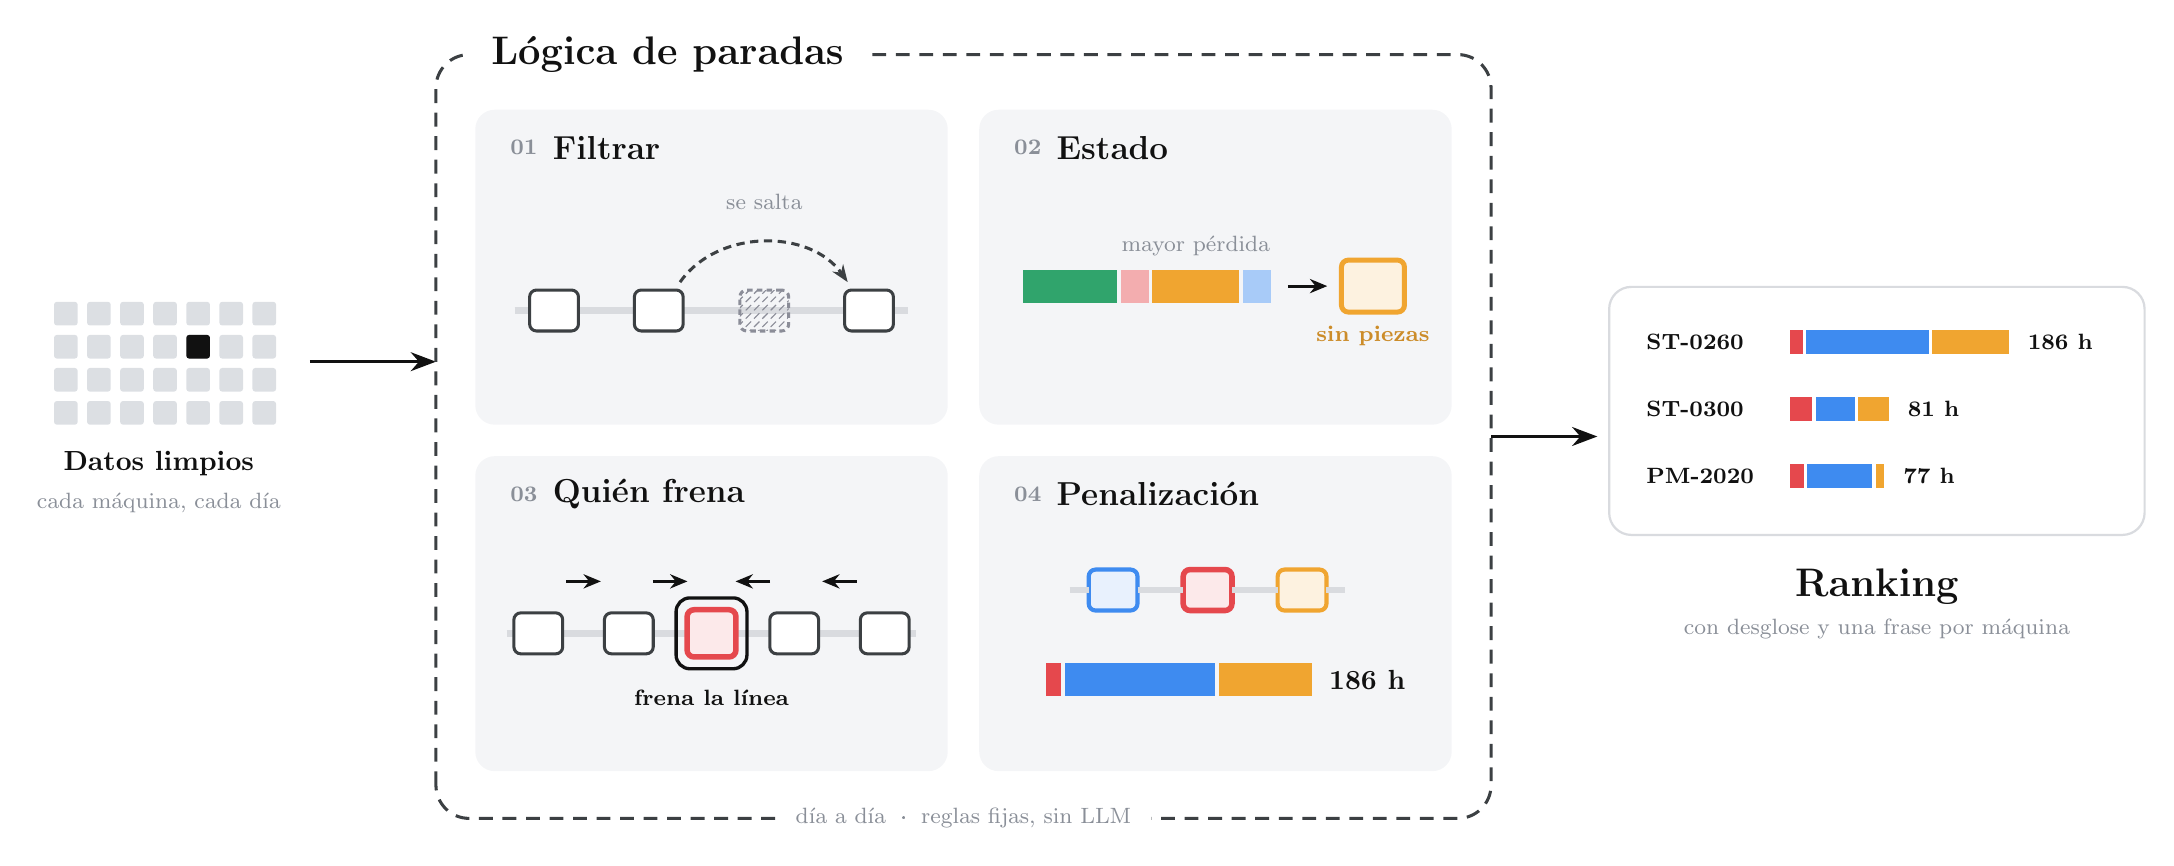
\begin{tikzpicture}[x=1cm,y=1cm]
  \def\TW{6.0}\def\TH{4.0}\def\G{0.4}\def\P{0.5}
  \def\BX{5.6}                         % borde izquierdo de la caja
  \pgfmathsetmacro{\BW}{2*\P+2*\TW+\G}
  \pgfmathsetmacro{\BH}{2*\P+2*\TH+\G+0.3}
  \pgfmathsetmacro{\BR}{\BX+\BW}
  \pgfmathsetmacro{\MY}{\BH/2}

  % --- Entrada: los datos limpios, una fila por máquina y día --------------------------------
  \foreach \i in {0,...,6} \foreach \j in {0,...,3}
    \fill[cell, rounded corners=1pt] (0.75+\i*0.42,\MY+0.15+\j*0.42) rectangle ++(0.3,0.3);
  \fill[ink, rounded corners=1pt] (0.75+4*0.42,\MY+0.15+2*0.42) rectangle ++(0.3,0.3);
  \node[font=\normalsize\bfseries\color{ink}] at (2.08,\MY-0.35) {Datos limpios};
  \node[font=\footnotesize\color{muted}] at (2.08,\MY-0.85) {cada máquina, cada día};
  \draw[flow] (4.0,\MY+0.95) -- (\BX,\MY+0.95);

  % --- La lógica: caja discontinua con los cuatro pasos ---------------------------------------
  \draw[ink2, line width=1.1pt, dash pattern=on 5pt off 3.5pt, rounded corners=12pt] (\BX,0) rectangle (\BR,\BH);
  \node[fill=white, inner xsep=7pt, font=\Large\bfseries\color{ink}, anchor=west] at (\BX+0.45,\BH) {Lógica de paradas};
  \node[fill=white, inner xsep=7pt, font=\footnotesize\color{muted}] at (\BX+\BW/2,0) {día a día \;·\; reglas fijas, sin LLM};

  % Fondo, número y título de cada paso. #1 columna, #2 fila (0 arriba), #3 número, #4 título
  \newcommand{\tile}[4]{%
    \pgfmathsetmacro{\tx}{\BX+\P+#1*(\TW+\G)}%
    \pgfmathsetmacro{\ty}{\P+0.1+(1-#2)*(\TH+\G)}%
    \fill[tile] (\tx,\ty) rectangle ++(\TW,\TH);
    \node[num] at (\tx+0.32,\ty+\TH-0.48) {#3};
    \node[head] at (\tx+0.86,\ty+\TH-0.48) {#4};
  }

  % 01 · Filtrar: una máquina sin dato fiable o fuera de servicio se salta y sus vecinas pasan a ser contiguas
  \tile{0}{0}{01}{Filtrar}
  \begin{scope}[shift={(\tx,\ty)}]
    \def\y{1.45}
    \draw[rule, line width=2.5pt] (0.5,\y) -- (5.5,\y);
    \node[machine] at (1.0,\y) {};
    \node[machine] at (2.33,\y) {};
    \node[machine, draw=nodata, pattern=north east lines, pattern color=nodata, dash pattern=on 2pt off 1.5pt] at (3.67,\y) {};
    \node[machine] at (5.0,\y) {};
    \draw[-{Stealth[length=2.2mm]}, line width=1.1pt, ink2, dash pattern=on 3pt off 2pt] (2.6,\y+0.36) to[bend left=55] (4.73,\y+0.36);
    \node[font=\footnotesize\color{muted}] at (3.67,\y+1.38) {se salta};
  \end{scope}

  % 02 · Estado: el color de cada máquina y día es su mayor pérdida
  \tile{1}{0}{02}{Estado}
  \begin{scope}[shift={(\tx,\ty)}]
    \def\y{1.55}
    \fill[work]           (0.55,\y) rectangle (1.75,\y+0.42);
    \fill[own!45]         (1.8,\y) rectangle (2.15,\y+0.42);
    \fill[starved]        (2.2,\y) rectangle (3.3,\y+0.42);
    \fill[blocked!45]     (3.35,\y) rectangle (3.7,\y+0.42);
    \node[font=\footnotesize\color{muted}] at (2.75,\y+0.72) {mayor pérdida};
    \draw[small arrow] (3.92,\y+0.21) -- (4.42,\y+0.21);
    \node[machine, draw=starved, line width=1.8pt, fill=starved!15, minimum width=8mm, minimum height=6.6mm] (m) at (5.0,\y+0.21) {};
    \node[font=\footnotesize\bfseries\color{starved!85!black}] at (5.0,\y-0.42) {sin piezas};
  \end{scope}

  % 03 · Quién frena: las flechas entre vecinas convergen en la máquina que frena la línea
  \tile{0}{1}{03}{Quién frena}
  \begin{scope}[shift={(\tx,\ty)}]
    \def\y{1.75}
    \draw[rule, line width=2.5pt] (0.4,\y) -- (5.6,\y);
    \foreach \x in {0.8,1.95,4.05,5.2} \node[machine] at (\x,\y) {};
    \draw[own, line width=2pt, fill=own!12, rounded corners=2.5pt] (2.69,\y-0.3) rectangle (3.31,\y+0.3);
    \draw[ink, line width=1.2pt, rounded corners=5pt] (2.55,\y-0.45) rectangle (3.45,\y+0.45);
    \foreach \c in {1.375,2.475} \draw[small arrow] (\c-0.22,\y+0.66) -- (\c+0.22,\y+0.66);
    \foreach \c in {3.525,4.625} \draw[small arrow] (\c+0.22,\y+0.66) -- (\c-0.22,\y+0.66);
    \node[font=\footnotesize\bfseries\color{ink}] at (3.0,\y-0.82) {frena la línea};
  \end{scope}

  % 04 · Penalización: sus horas propias más lo que hace perder a sus vecinas los días que frena
  \tile{1}{1}{04}{Penalización}
  \begin{scope}[shift={(\tx+0.3,\ty)}]
    \def\y{2.3}
    \node[machine, draw=blocked, line width=1.5pt, fill=blocked!12] at (1.4,\y) {};
    \node[machine, draw=own, line width=2pt, fill=own!12] at (2.6,\y) {};
    \node[machine, draw=starved, line width=1.5pt, fill=starved!15] at (3.8,\y) {};
    \draw[rule, line width=2.5pt] (0.85,\y) -- (1.09,\y) (1.71,\y) -- (2.29,\y) (2.91,\y) -- (3.49,\y) (4.11,\y) -- (4.35,\y);
    \def\b{0.95}
    \fill[own]     (0.55,\b) rectangle ++(0.19,0.42);
    \fill[blocked] (0.79,\b) rectangle ++(1.9,0.42);
    \fill[starved] (2.74,\b) rectangle ++(1.18,0.42);
    \node[font=\normalsize\bfseries\color{ink}, anchor=west] at (4.02,\b+0.21) {186 h};
  \end{scope}

  % --- Salida: el ranking con su desglose ----------------------------------------------------
  \pgfmathsetmacro{\OX}{\BR+1.5}
  \def\OW{6.8}
  \pgfmathsetmacro{\OY}{\MY-1.25}
  \fill[white, draw=rule, line width=0.8pt, rounded corners=8pt] (\OX,\OY) rectangle ++(\OW,3.15);
  \foreach \k/\op/\o/\p/\n/\t in {0/ST-0260/10.9/107.9/66.8/186, 1/ST-0300/19.4/34.7/26.5/81, 2/PM-2020/11.7/57.5/7.5/77} {
    \pgfmathsetmacro{\ry}{\OY+2.45-\k*0.85}
    \pgfmathsetmacro{\s}{2.7/186}
    \node[font=\footnotesize\bfseries\color{ink}, anchor=west] at (\OX+0.35,\ry) {\op};
    \pgfmathsetmacro{\xa}{\OX+2.3}
    \pgfmathsetmacro{\xb}{\xa+\o*\s}
    \pgfmathsetmacro{\xc}{\xb+0.04+\p*\s}
    \pgfmathsetmacro{\xd}{\xc+0.04+\n*\s}
    \fill[own] (\xa,\ry-0.15) rectangle (\xb,\ry+0.15);
    \fill[blocked] (\xb+0.04,\ry-0.15) rectangle (\xc,\ry+0.15);
    \fill[starved] (\xc+0.04,\ry-0.15) rectangle (\xd,\ry+0.15);
    \node[font=\footnotesize\bfseries\color{ink}, anchor=west] at (\xd+0.12,\ry) {\t\ h};
  }
  \node[font=\Large\bfseries\color{ink}] at (\OX+\OW/2,\OY-0.65) {Ranking};
  \node[font=\footnotesize\color{muted}] at (\OX+\OW/2,\OY-1.2) {con desglose y una frase por máquina};
  \draw[flow] (\BR,\MY) -- (\OX-0.15,\MY);
\end{tikzpicture}
\end{document}
